\chapter{微软Edx语音识别笔记}
本章笔记主要是对微软Edx的课程\href{https://courses.edx.org/courses/course-v1:Microsoft+DEV287x+1T2019a/course/}{Speech Recognition System}的记录,首版主要是翻译,再加上自己翻阅其他资料综合起来的一些思考和总结。代码见\href{https://github.com/MicrosoftLearning/Speech-Recognition}{Speech-Recognition}
\section{Background and Fundamentals}

\subsection{Phonetics} % (fold)
\label{ssub:phonetics}
Phonetics(语音学)是Linguistics(语言学)的一个分支,其研究的是人类语音发出的声音(sound)。语音学围绕着声音的产生(通过人类的发音器官)、声音的声学特性和感知。语音学有三个基本的分支,这三个分支都与ASR有关系。
\begin{enumerate}
	\item Articulatory Phonetics(发音语音学):通过发音器官、不同说话人而产生的声音;
	\item Acoustic Phonetics(声学语音学):声音从说话人到听者的传输;
	\item Auditory Phonetics(听觉语音学):听者对于声音的接收和感知。
\end{enumerate}

声音的最小单元我们成为\textcolor{red}{Phoneme},即音素。序列中的词(Words)是由一个或多个音素组成的。一个音素的声学实现称为\textcolor{red}{Phone}。图\ref{fig:exam-phonemes}展示了美式英语的音素和一般实现办法。
\begin{figure}[htbp]
  \centering
  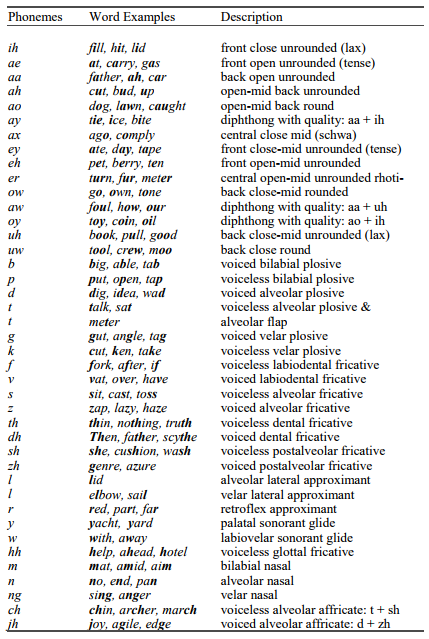
\includegraphics[width=0.35\textwidth]{phonemes}
  \caption{美式英语的音素和一般实现办法 \label{fig:exam-phonemes}}
\end{figure}

一般我们将音素分为两类:元音(Vowel)和辅音(Consonants)。
\begin{enumerate}
	\item Vowels:元音有两个特点,一是元音都是发声的声音(voiced sound),这意味着从声带(vocal chords)到口腔(mouth cavity)的气流是由声带的某种基频的震动(或者音高)产生的。二是舌头在生产过程中不会以任何方式形成气流收缩。每个元音发声的时候舌头、嘴唇和下巴的造型都不一样。这些不同的方式形成了不同的共振态,我们称之为共振峰。这些共振峰的共振态频率形成了不同的元音。
	\item Consonants:辅音是通过在口腔中或者空气中很明显的气流收缩形成的。有些辅音和元音一样是发声的,有些是不发声的。不发声的音素不会激活声带,因此也不存在基频或者音高。一些辅音音调成对出现,只有在有声或无声的情况下才有所不同,但在其他方面是相同的。比如说/b/和/p/这两个音素的发音方式是相同的,因为你的嘴唇、下巴还有舌头的姿势是一样的。但是/b/是发声的,/p/是不发声的。
\end{enumerate}

音素的另外一个重要特性是\textcolor{red}{其根据不同的上下文音素发音是会改变的}。我们称之为Phonetic Context。之所以会这样,是因为协同发音(coarticulation)。这些声音连续起来发音会改变其原有的特征。由协同发音产生的音素我们称为音素变体(allophones)。

所有当前的这些语音识别系统都使用了音素的语境相关的特性来建立处于不同phonetic context的音素模型。
% subsubsection phonetics (end)

\subsection{Words and Syntax} % (fold)
\label{sub:words_and_syntax}
Syllable 是一串声音,是个序列,由一个核心的音素,可能有初始音素和终止音素,这个核心音素一般是个元音或者一个音节辅音(syllablic consonant),是能够唱出来或者吼出来的声音。

举个例子,英文单词 "bottle" 包含两个 syllable 。第一个 syllable 有三个 phone ,在 Arpabet 音素描述代码里,是 "b aa t" 。这个 "aa" 就是核心音素,"b" 是发声的初始音素,"t" 是不发音的终止音素;第二个 syllable 是只包含一个 syllablic cosonant "l"。

一个 syllable 也可以组成一个词,其本身就是一个单独的音素,比如说,"Eye","uh",或者"eau"(医:水)。

语音识别里面,syllable 很少会考虑作为声学模型的建模单元,而词一般是变成音素来建模。

Syntax(句法规则)描述了给定词和定义了语法的规则下,句子的形成。而 Semantics(语义学)一般指代的是句子中的词或者短语是如何形成句意的。Syntax 和 Semantics 是 NLP 的重要组成部分,但是在语音识别里面,不起主要作用。
% subsection words_and_syntax (end)

\subsection{Measuring Performance} % (fold)
\label{sub:measuring_performance}
在语音识别系统的搭建和实验中,如何来衡量一个系统的好坏呢?由于语音识别是一个序列任务,跟图像当中的分类不一样,因此我们在衡量系统的性能时需要考虑到整个序列。

语音识别准确率衡量最常用的一个指标是词错误率(word error rate,WER)。一般识别出来的结果可能会产生三种错误:替换(substitution)、删除(delete)和插入(insert)。替换指的是一个词被识别成了另外一个词;删除指的是原本有词,但是没有识别出来;插入指的是原本没有词,多识别出来了词。WER 的计算方式如公式\ref{eqn:wer}。
\begin{align}
\label{eqn:wer}
  WER = \frac{N_{sub}+N_{ins}+N_{del}}{N_{ref}}
\end{align}
其中$N_{sub}$、$N_{ins}$和$N_{del}$分别是替换、插入和删除的数量,而$N_{ref}$是参考文本描述中词的个数。

WER的计算用的是通过计算实际输出描述和参考文本描述之间的\href{https://en.wikipedia.org/wiki/Edit_distance}{字符串编辑距离}得到的。编辑距离的实现通过动态规划算法。因为长文本的编辑距离可能不可靠,所以我们通过逐句的计算累积的错误,这些错误最终整合到一起来计算测试集的WER。

表\ref{tab:wer}呈现了实际输出和参考文献之间的不同,以及对应的三种错误。
\begin{lstlisting}[language = python, numbers=left, 
         numberstyle=\tiny,keywordstyle=\color{blue!70},
         commentstyle=\color{red!50!green!50!blue!50},frame=shadowbox,
         rulesepcolor=\color{red!20!green!20!blue!20},basicstyle=\ttfamily]
Ref: however a little later we had a comfortable chat
Hyp: how never a little later he had comfortable chat
\end{lstlisting}
\begin{table}[h]
 \centering
 \caption{struct中常用的数据类型、C语言的对应类型和占用字节数}
   \begin{tabular*}{1\textwidth}{@{\extracolsep{\fill}}ccc}
   \toprule
    {\bf Reference} & {\bf Hypothesis} & {\bf Error} \\
   \midrule
   however      &        how  & Substitution \\ \hline
                &      never  &  Insertion   \\ \hline
         a      &          a  &              \\ \hline
    little      &     little  &              \\ \hline
    later       &      later  &              \\ \hline
    we          &         he  & Substitution  \\ \hline
    had         &        had  &              \\ \hline
    a           &             &   Deletion   \\ \hline
	comfortable & comfortable &              \\ \hline
      chat &       chat       &              \\
   \bottomrule
   \end{tabular*}%
 \label{tab:wer}%
\end{table}%

在某些情况中,这三种错误的成本不对等,那么计算编辑距离的时候可以作相应的调整。

句错误率(Sentence Error Rate,SER)是另外一种衡量系统的标准,其计算方式是整句没有出现任何错误。SER 仅仅作为一个指标,来看下错误的句子占全部句子的比例。

% subsection measuring_performance (end)

\subsection{Significance Testing} % (fold)
\label{sub:significance_testing}
统计显著性检验(statistical significance testing)涉及测量两个实验(或算法)之间的差异在多大程度上归因于两个算法中的实际差异,或者仅仅是数据,实验设置或其他因素中的结果固有变异性。统计显著性是所有分类任务的基石,只是统计显著性检验的方法取决于任务的特性。大多数方法的核心是假设检验的概念中存在一个无效假设。问题在于你有多大的confidence能够说无效假设会被拒绝。

对于语音识别来说,比较两个实验或者算法最常用的方法是 Matched Pairs Sentence-Segment Word Error(MAPSSWE)检验,简称为 Matched Pairs Test\upcite{asr-sign}。

在这个方法中,测试集被分为几份,假设这些子测试集中任意一个的错误都与其他子测试集统计独立。这个假设和语音识别的实验很贴合,因为测试数据都是一句一句的经由识别器输出结果。给定了每一个句子的WER,就很容易构建一个matched pairs\upcite{Pallet1990Tools}。
% subsection significance_testing (end)

\subsection{Other Consideration} % (fold)
\label{sub:other_consideration}
除去准确率,对识别系统性能的影响还可能包括计算需求,处理速度或者延迟什么的。解码速度一般用实时因子(real-time factor,RTF)来衡量。RTF为1.0指的是系统处理10s的数据需要花10s的时间。

RTF高于1.0意味着系统要花更多的时间来解码,对于某些应用,也许是可以接受的,比如希望获得一个会议或者讲座的转写,相对于快速的得到转写结果,准确率可能更重要一些,因此多花一些时间也是可以接受的。

当RTF低于1.0,系统会在当前数据达到前就处理好了之前的数据。当不止一个系统在同一个机器上运行的时候,这个就比较有用了。在这种情况下,我们可以用多线程来并行处理多路音频流。此外RTF低于1.0意味着系统能够满足在线实时解码的音频流应用。比如说,当我们在处理一个手机上远程音频需求的时候,网络阻塞可能会使得服务器接收音频产生间隙和延迟。如果语音识别器能够以比实时更快的速度来处理,那么它就可以在数据达到之后迅速跟进,追上最新的音频进度,以速度来掩盖网络的延迟。

一般来说,语音识别系统能够在准确率和速度之间调整,但是这种调整也是有限的,不可能无限好或者无限快。对于一个给定的模型和测试集,speed-accuracy图有一条不可被突破的渐近线(asymptote),即便给予无限的算力。所以准确率是有个极限的,这个时候的错误率可以认为就是模型带来的错误。一旦根据模型搜索找到了最好的结果,进一步的处理也不会带来准确率上的提升。
% subsection other_consideration (end)

\subsection{The Fundamental Equation} % (fold)
\label{sub:the_fundamental_equation}
语音识别可以看作一个优化任务。特别地,给定一个观测序列$O=\{O_{1},...,O_{N}\}$,我们找寻的是最有可能的词序列$W=\{W_1,...,W_M\}$,也就是说我们要找到最大化后验概率$P(W|O)$的词序列,如公式\ref{eqn:fundamental-equation}。
\begin{align}
\label{eqn:fundamental-equation}
  \hat{W} = \arg\mathop{\max}_{W} P(W|O)
\end{align}
利用贝叶斯规则,我们得到公式\ref{eqn:fun-bayes}。
\begin{align}
\label{eqn:fun-bayes}
  P(W|O) = \frac{P(W)P(O|W)}{P(O)}
\end{align}

因为词序列并不依赖于观测序列的边缘概率分布$P(O)$,我们可以忽略这个部分,综合上述两个公式,我们得到公式\ref{eqn:fun-final}。
\begin{align}
\label{eqn:fun-final}
  \hat{W} = \arg\mathop{\max}_{W} P(W)P(O|W)
\end{align}

这就是语音识别的基本公式。语音识别问题就可以看作是在这个联合模型上的搜索。

公式中的$P(O|W)$叫做\textcolor{red}{声学模型(acoustic model)}。这个模型描述了在给定词序列$W$的条件下,声学观测$O$的分布。声学模型表征的是词序列是如何转换成声学实现的,进而转换成ASR系统的声学观测的。

公式中的$P(W)$叫做\textcolor{red}{语言模型(language model)},其只取决于词序列$W$。语言模型给每一个可能的词序列一个概率值。它是由日常使用的一些词序列训练成的。一个训练好的英语语言模型会给"I like turtles"高的概率值,给"Turtles sing table"低的概率值。语言模型促使着词序列的搜索沿着训练数据中的模式开展。语言模型也可以在一些纯文本的应用中见到,比如浏览器的自动补全等。

由于诸多原因,构建一个语音识别系统比这个简单地公式所能呈现的要复杂的多得多。
% subsection the_fundamental_equation (end)
\subsection{Lab 1} % (fold)
\label{sub:lab-1}
本模块有一个实验作业,标题为"Create a speech recognition scoring program"。

{\bf Required files:}
\begin{itemize}
	\item \textcolor{blue}{wer.py}
	\item \textcolor{blue}{M1\_score.py}
\end{itemize}}

{\bf Instructions:}

In this lab, you will write a program in Python to compute the word error rate (WER) and sentence error rate (SER) for a test corpus. A set of hypothesized transcriptions from a speech recognition system and a set of reference transcriptions with the correct word sequences will be provided for you.

This lab assumes the transcriptions are in a format called the "trn" format, created by NIST. The format is as follows. The transcription is output on a single line followed by a single space and then the root name of the file, without any extension, in parentheses. For example, the audio file "tongue\_twister.wav" would have a transcription

sally sells seashells by the seashore (tongue\_twister)

Notice that the transcription does not have any punctuation or capitalization, nor any other formatting (e.g. converting "doctor" to "dr.", or "eight" to "8"). This formatting is called "Inverse Text Normalization" and is not part of this course.

The python code \textcolor{blue}{M1\_Score.py} and \textcolor{blue}{wer.py} contain the scaffolding for the first lab. A main function parses the command line arguments and string\_edit\_distance() computes the string edit distance between two strings.

Add code to read the trn files for the hypothesis and reference transcriptions, to compute the edit distance on each, and to aggregate the error counts. Your code should report:
\begin{itemize}
	\item Total number of reference sentences in the test set
	\item Number of sentences with an error
	\item Sentence error rate as a percentage
	\item Total number of reference words
	\item Total number of word errors
	\item Total number of word substitutions, insertions, and deletions
	\item The percentage of total errors (WER) and percentage of substitutions, insertions, and deletions
\end{itemize}

The specific format for outputting this information is up to you. Note that you should not assume that the order of sentences in the reference and hypothesis trn files is consistent. You should use the utterance name as the key between the two transcriptions.

When you believe your code is working, use it to process hyp.trn and ref.trn in the misc directory, and compare your answers to the solution.

% subsection lab (end)

\section{Speech Signal Processing}

\section{Acoustic Modeling}

\section{Language Modeling}

\section{Speech Decoding}

\section{Advanced Acoustic Modeling}